
\chapter{Modelos Compartimentais}
\label{sec-modelos-compartimentais}

Neste cápitulo são apresentados os principais conceitos acerca dos modelos compartimentais
para a compreensão do trabalho desenvolvido nesta dissertação. No fim do cápitulo
é apresentada uma pequena revisão de aplicação de PINNs com modelos compartimentais.

\section{Origens}

Apresnetado no conjunto de trabalhos seminais \cite{kermack-mcKendrick:1927}, 
\cite{kermack-mcKendrick-pt2:1932} e \cite{kermack-mcKendrick-pt3:1933} e consolidados
em estudos como \cite{kendall:2023-modelos-epd-estocasticos}, 
modelos Compartimentais nada mais são do que modelos epidemiológicos utilizados 
no estudo de doenças contagiosas que separam a população em grupos.
Os fluxos de indivíduos entre esses grupos, chamados de compartimentos, são modelados 
por meio de operações de diferenciação.

\section{O modelo SIR}

Apresentado no trabalho seminal de \cite{kermack-mcKendrick:1927}, 
o modelo \textit{SIR} (Susceptible-Infected-Recovered) é definido pelo conjunto 
de equações \ref{eq:SIR-1}, \ref{eq:SIR-2} e \ref{eq:SIR-3}.

\begin{eqnarray}\label{eq:sir}
   \frac{dS(t)}{dt} &=& \frac{-\beta S(t)}{N} I(t),  \quad t > t_0, \label{eq:SIR-1}\\
   \frac{dI(t)}{dt} &=& \frac{\beta S(t)}{N} I(t) - \gamma I(t), \quad t > t_0, \label{eq:SIR-2}\\
   \frac{dR(t)}{dt} &=& \gamma I(t),  \quad t > t_0, \label{eq:SIR-3}
\end{eqnarray}

Estas três equações formam um sistema de equações diferencias de fácil interpretação.
A primeira equação modela a iteração entre pessoas infectadas e pessoas suscetíveis,
o parâmetro $\beta$, a taxa de infecção, diz quantos destes encontros resultaram 
em novos casos da doença. 
A terceira equação modela a recuperação de individuos ao
longo do tempo, o parâmetro $\gamma$ é taxa de individuos que se recuperam por 
unidade de tempo, sendo que a recuperação pode ser a cura da doença ou o falecimento
do individuo, já que o \textit{SIR} não distinguir os dois casos. 
A segunda equação é a soma do primeira e da terceira equação, mas com seus sinais
trocados. Ela modela o fluxo de indivíduos que entram e saem do compartimento
de infectados.  

Por se tratar de um sistema de equações diferencias ordinárias com três equações,
são necessárias três condições iniciais para se obter um problema de valor
inicial.

\begin{eqnarray}
   S(0) &=& S_0 \label{eq:SIR-S0}\\
   I(0) &=& I_0 \label{eq:SIR-I0}\\
   R(0) &=& R_0 \label{eq:SIR-R0}
\end{eqnarray}

Como o modelo não inclui mortes naturais ou por outras causas que não a doença
que está sendo modelada, nem o nascimento de pessoas na população estuda, assume-se
que a soma dos três comparimentos para qualquer tempo $t$ é igual ao total 
$N$ da popuiação,

\begin{equation}
   S(t) + I(t) + R(t) = N,  \quad t > t_0, \label{eq:SIR-4}
\end{equation}

O modelo pode ser entendido com um grafo em que os individuas fluem de um 
compartimento para outro a uma taxa $\beta$ e $\gamma$. 
A figura \ref{fig:sir-grafo} representa o \textit{SIR} por esta perspectiva.

\begin{figure}
\centering
\begin{tikzpicture}[
    node distance=2.5cm,
    box/.style={rectangle, minimum width=2cm, minimum height=1.5cm, 
                draw=black, thick, align=center, rounded corners=5pt,
                font=\large\bfseries},
    arrow/.style={-Stealth, thick, line width=1.2pt},
    label/.style={midway, sloped, font=\small}
]

    % Define nodes
    \node[box, fill=blue!20] (S) {Susceptible \\ S(t)};
    \node[box, fill=red!20, right=of S] (I) {Infected \\ I(t)};
    \node[box, fill=green!20, right=of I] (R) {Recovered \\ R(t)};

    % Transitions
    \draw (S) edge[->] node[label,above] {$\beta$} (I);
    \draw (I) edge[->] node[label,above] {$\gamma$} (R);

\end{tikzpicture}
\caption{Grafo para o \textit{SIR}. Fonte: elaborada pelos autores.}
\label{fig:sir-grafo}
\end{figure}

Certas definições são necessárias neste ponto para se compreender os modelos compartimentais. 
Em modelos epidemiológicos, incidência é o fluxo de novos casos por unidade de tempo,
enquanto que a prevalência é a quantidade de casos na população num instante $t$.
No caso do \textit{SIR}, estes conceitos são representados respectivamente pelo
termo $\frac{-\beta S(t)}{N}$ e pela equação $I(t)$. 

O número de reprodução básico $R_0$ é defido como a relação entre os parametros
$\beta$ e $\gamma$. Ele é de particular interesse para o estudo da propagação
de uma doença, pois se $R_0 > 1$, significa que a dispersão da doença
ainda está em curso e o número de infectados tende a aumentar. 
Se $R_0 < 1$, significa que a dispersão já atigiu seu pico e o número de individuos
infectados tender a diminuir. Se $R_0 = 1$ a doença está em equilíbrio e o número 
de infectados tender a se manter o mesmo.

\begin{equation}\label{eq:numero-reproducao-basico}
    R_0 = \frac{\beta}{\gamma}
\end{equation}

Um valor relacionado ao número de reprodução básico $R_0$, é o número de reprodução
efetivo $R_e$. Enquanto que o número de reprodução básico $R_0$ é utilizado para
medir o dispersão de uma doença no início de uma pandemia. 
Seu valor é obtido pela multiplicação de $R_0$ por $S$ num instante $t$.

\begin{equation}\label{eq:numero-reproducao-efetivo}
    R_e = R_0 S(t)
\end{equation}

O limite $\mathcal{T}$ define o valor máximo de indivíduos que estarão contaminados
no pico da pandemia. Este limite é importante para tomadores de decisão e governos
para entender os efeitos sobre os serviços de saúde pública.

\begin{equation}
    \mathcal{T} = \frac{\gamma}{\beta}N = \frac{N}{R_0}
\end{equation}

A figura \ref{fig:exemplo-sir} mostra um exemplo do \textit{SIR} com $\beta=0.8$
e $\gamma=0.1$ e as três curvas características desse modelo.

\begin{figure}[htpb]
\centering
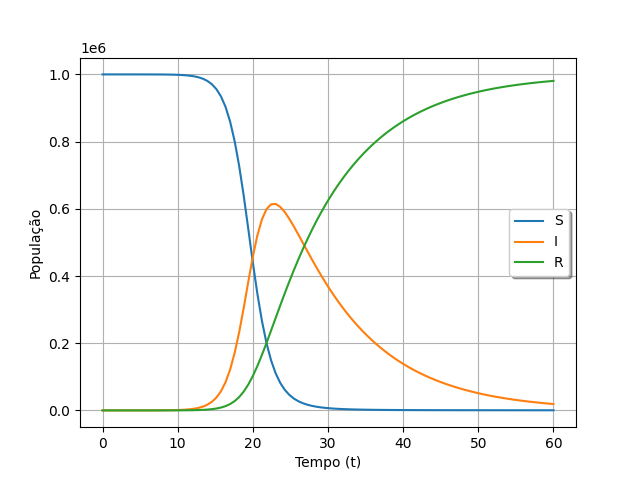
\includegraphics[width=0.6\textwidth]{figuras/sir-example-beta0.8-gamma0.1.png}
\caption{Exemplo do SIR com $\beta=0.8$ e $\gamma=0.1$.}
\label{fig:exemplo-sir}
\end{figure}

\section{Pontos de equilíbrio}

Os modelos compartimentais possuem dois pontos de equilíbrio chamados de 
ponto de equilíbrio livre de doenças (\textit{Deacese Free Equilibrium}) e 
ponto de equilíbrio endemico (\textit{Endemic Equilibrium}). 
O primeiro ponto é atingido quando não há mais indivíduos infectados na população,
ou seja, nos ponto em que $I$ é igual a zero. O ponto de equilíbrio endêmico
é atigindo justamente quando o número de novos casos é compensado pelo número
de indivíduos que se recuperam, mantendo o número de indivíduos no compartimento
\textit{Infected} constante, mas diferente de zero.

\section{Pontos críticos}

Utilizando o foi desenvolvido na seção anterior, pode-se facilmente encontrar os 
pontos críticos do modelo SIR. Considerando que os pontos de equilíbrio do modelo 
SIR são determinados pela solução do sistema composto pelas equações
\ref{eq:SIR-pontos-criticos-1}, \ref{eq:SIR-pontos-criticos-2} e \ref{eq:SIR-pontos-criticos-3}.

\begin{eqnarray}
    -\beta SI &=& 0 \label{eq:SIR-pontos-criticos-1}\\
    \beta SI - \gamma I &=& 0 \label{eq:SIR-pontos-criticos-2}\\
    \gamma I &=& 0 \label{eq:SIR-pontos-criticos-3}
\end{eqnarray}

A última equação $\gamma I=0$ implica que $I=0$. Substituindo este valor na primeira e 
segunda equações, as equações são satisfeitas para qualquer valor de S. 
Portanto, o sistema tem um conjunto de pontos de equilíbrio da forma:

\begin{equation}\label{eq:sir-conjunto-solucoes-eq-livre-doenca}
    (S* , I*, R*) = (S* , 0, R*)    
\end{equation}

Sendo $S* + R* = N$, ou seja, qualquer ponto em que não haja infectados e a soma 
dos suscetíveis e recuperados seja igual a N representa um estado de equilíbrio. 
Isso significa que o sistema pode estabilizar-se em diferentes estados dependendo 
da quantidade de indivíduos que permaneceram suscetíveis ou que foram recuperados. 
Esse é o estado de equilíbrio livre de doença, onde toda 
população está no compartimento \textit{Susceptible} ou \textit{Recovered} e não 
há mais infectados.

A análise de estabilidade dos pontos de equilíbrio do modelo SIR pode ser facilmente 
feita através da matriz jacobiana do sistema de equações diferencias. 
Considere a matriz \ref{eq:jacobiana-sir}.

\begin{equation}\label{eq:jacobiana-sir}
J(S,I,R) = 
\begin{pmatrix}
\frac{\partial f_1}{\partial S} & \frac{\partial f_1}{\partial I} & \frac{\partial f_1}{\partial R} \\[0.5em]
\frac{\partial f_2}{\partial S} & \frac{\partial f_2}{\partial I} & \frac{\partial f_2}{\partial R} \\[0.5em]
\frac{\partial f_3}{\partial S} & \frac{\partial f_3}{\partial I} & \frac{\partial f_3}{\partial R}
\end{pmatrix}
=
\begin{pmatrix}
-\beta I & -\beta S & 0 \\
\beta I & \beta S - \gamma & 0 \\
0 & \gamma & 0
\end{pmatrix}
\end{equation}

Utilizando a equação \ref{eq:sir-conjunto-solucoes-eq-livre-doenca} e aplicando-a
na matriz \ref{eq:jacobiana-sir}, chega-se ao ponto de equilíbrio 
\ref{eq:equilíbrio-sir}.

\begin{equation}\label{eq:equilíbrio-sir}
J(S*,0,R*)
=
\begin{pmatrix}
0 & -\beta S & 0 \\
0 & \beta S - \gamma & 0 \\
0 & \gamma & 0
\end{pmatrix}
\end{equation}

Os autovalores dessa matriz são $\gamma_1=0$, $\gamma_2=0$, $\gamma_3=\beta S* - \gamma$. 
Isso significa que para $S* < \gamma \beta$ tem-se $\gamma_3 < 0$ e a solução 
de equilíbrio é estável.

\section{Matriz de nova geração}

Uma forma de se calcular o número de reprodução básico $R_0$ é a aplicar a técnica
de matriz de nova geração. Proposta por \cite{diekmann:1990-matriz-de-nova-geracao},
o método consiste em 

\begin{itemize}
    \item Divida toda a popuiação em $n$ compartimentos de tamanho $m$ tal que 
    $m < n$.

\end{itemize}

Aplicando o método descrito acima para o modelo \textit{SIR} obtem-se as seguintes
definições:

\begin{equation}
\frac{dI}{dt} = \underbrace{\beta SI}_{\mathcal{F}} - \underbrace{\gamma I}_{\mathcal{V}}
\end{equation}

\begin{equation}
F = \frac{\partial \mathcal{F}}{\partial I} = \beta S\big|_{DFE} = \beta N, \quad 
V = \frac{\partial \mathcal{V}}{\partial I} = \gamma
\end{equation}

\begin{equation}
FV^{-1} = (\beta N)\left(\frac{1}{\gamma}\right) = \frac{\beta N}{\gamma}
\end{equation}

\begin{equation}
R_0 = \rho(FV^{-1}) = \frac{\beta N}{\gamma}
\end{equation}


\section{Identificabilidade de um Modelo}

Uma questão pertinente a modelos baseados em equações diferencias é a 
identificabilidade. A identificabilidade está relacionada a capacidade de 
estabelecer os parâmetros de um modelo de forma única com base nos dados disponíveis
e independente das condições iniciais. Há dois tipos de identificabilidade:
\begin{itemize}
    \item \textbf{Identificabilidade estrutural:} Refere-se a capacidade de estabelecer
    os parâmetros de um modelo utilizando dados ideias. Isto é, desprovidos de ruídos
    e lacunas e dispersos de forma uniforme pelo domínio do problema. 
    \item \textbf{Identificabilidade prática:} Refere-se a capacidade de estabelecer
    os parâmetros de um modelo utilizando dados reais que possuem ruído, lacunas 
    (não foram coletados em todos os dias da semana, por exemplo) ou não estão uniformemente
    distribuídos pelo domínio do problema (há mais dados referentes a uma semana epidemiológica
    do outra).
\end{itemize}
A análise dos dois tipos de identificabilidade é importante para o estudo de 
modelos compartimentais. No primeiro caso para o estudo teórico de modelos 
compartimentais, mais especificamente, para demonstrar teoricamente ser possível 
estimar parâmetros como $\beta$, $\gamma$ e $\alpha$ de novas propostas de modelos 
compartimentais utilizando métodos analíticos como álgebra diferencial e 
expansões por séries de Taylor. 
No segundo caso para lidar como dados epidemiológicos reais e ter garantias que os
parâmetros estimados para o modelo têm algum grau de confiabilidade. As técnicas
mais comuns para se obter os parâmetros a partir de um conjunto de dados são os 
métodos não-paramétricos como \textit{bootstrapping} e simulações de Monte Carlo, 
além de outras técnicas estatísticas como matrizes de informação de \textit{Fisher}.  

% \begin{equation}\label{eq:matriz-de-infor-fisher}
%     F(\mathbf{p}) = E\left[\left(\frac{\partial \log L}{\partial \mathbf{p}}\right)^T \left(\frac{\partial \log L}{\partial \mathbf{p}}\right)\right]
% \end{equation}

Formalmente, um problema de identificabilidade pode ser expresso pelas equações
\ref{eq:problema-identificabilidade-1} e \ref{eq:problema-identificabilidade-2}.
Sendo $\mathbf{p}$ um conjunto de parâmetros, o problema de identificabilidade
consiste em determinar se $\mathbf{p} \rightarrow \mathbf{y}$ é injetivo. 

\begin{eqnarray}
\frac{d\mathbf{x}}{dt} &=& f(\mathbf{x}, \mathbf{p}, t) \quad \text{Equações de estado} \label{eq:problema-identificabilidade-1}\\
\mathbf{y} &=& h(\mathbf{x}, \mathbf{p}, t) \quad \text{Equações de observação} \label{eq:problema-identificabilidade-2}
\end{eqnarray}

Um dos fatores mais importantes para determinar a identificabilidade de um modelo
compartimental são as condições iniciais. O que cria um problema para a aplicação
desses modelos sob qualquer situação, pois geralmente, não se sabe as condições
inicias reais.

\section{Análise de Sensibilidade}

Partial Rank Correlation Coefficients (PRCC)

\section{Problemas Inversos}

Por ser tratarem de problemas de valor inicial, os problemas envolvendo modelos 
compartimentais podem ser facilmente resolvidos por meio de métodos numéricos 
tradcionais, porém quando se deseja resolver um problema inverso envolvendo modelos
compartimentais, ou seja, descobrir parâmetros como $\beta$ e $\gamma$ a partir
de um conjunto de dados, deve se considerar que problemas inversos são mal-postos.
Cabe aqui prover uma formalização do que são problemas bem postos e mal postos.

Um problema é considerado bem-posto se apresentar as seguintes 3 condições:

\begin{itemize}
    \item \textbf{Existência}: Existe ao menos uma solução. 
    \item \textbf{Unica}: Há no máximo uma solução.
    \item \textbf{Estável}: A solução depende continuamente nos dados.  
\end{itemize}

Enquanto que problemas diretos são considerados bem postos, problemas inversos 
são mal-postos. O motivo é que problemas inversos não satisfazem o segundo critério,
há mais de uma solução possível para um problema inverso.

\section{Adicionando Compartimentos}

Baseados no modelo \textit{SIR}, foram propostos outros modelos com mais 
compartimentos, como o \textit{SIRD} (Susceptible-Infected-Recovered-Deacesed) 
\cite{giles:77-sird} que separa o compartimento de \textit{Recovered} em dois, um
para os indivíduos que se recuperaram (R) e outro para os que vieram a falecer devido
a doença (D).

\begin{figure}
\centering
\begin{tikzpicture}[
    node distance=2.5cm,
    box/.style={rectangle, minimum width=2cm, minimum height=1.5cm, 
                draw=black, thick, align=center, rounded corners=5pt,
                font=\large\bfseries},
    arrow/.style={-Stealth, thick, line width=1.2pt},
    label/.style={midway, sloped, font=\small}
]

    % Define nodes
    \node[box, fill=blue!20] (S) {Susceptible \\ S(t)};
    \node[box, fill=red!20, right=of S] (I) {Infected \\ I(t)};
    \node[box, fill=green!20, right=of I] (R) {Recovered \\ R(t)};
    \node[box, fill=orange!20, right=of I, above=of R] (D) {Deacesed \\ D(t)};

    % Transitions
    \draw (S) edge[->] node[label,above] {$\beta$} (I);
    \draw (I) edge[->] node[label,above] {$\gamma$} (R);
    \draw (I) edge[->] node[label,above] {$\alpha$} (D);

\end{tikzpicture}
\caption{Grafo para o \textit{SIRD}. Fonte: elaborada pelos autores.}
\label{fig:sird-grafo}
\end{figure}

Outro exemplo é o \textit{SEIR} que inclui um compartimento para individuos que 
foram expostos a doença, mas ainda não manifestaram sintomas, ele é aplicável a 
doenças que possuem um tempo de latência entre o contanto com patogêneo e o surgimento
dos sintomas e capacidade do indivíduo de transmitir a doença. 

\begin{figure}
\centering
\begin{tikzpicture}[
    node distance=1.5cm,
    box/.style={rectangle, minimum width=2cm, minimum height=1.5cm, 
                draw=black, thick, align=center, rounded corners=5pt,
                font=\large\bfseries},
    arrow/.style={-Stealth, thick, line width=1.2pt},
    label/.style={midway, sloped, font=\small}
]

    % Define nodes
    \node[box, fill=blue!20] (S) {Susceptible \\ S(t)};
    \node[box, fill=orange!20, right=of S] (E) {Exposed \\ E(t)};
    \node[box, fill=red!20, right=of E] (I) {Infected \\ I(t)};
    \node[box, fill=green!20, right=of I] (R) {Recovered \\ R(t)};

    % Transitions
    \draw (S) edge[->] node[label,above] {$\beta$} (E);
    \draw (E) edge[->] node[label,above] {$\gamma$} (I);
    \draw (I) edge[->] node[label,above] {$\alpha$} (R);

\end{tikzpicture}
\caption{Grafo para o \textit{SIRD}. Fonte: elaborada pelos autores.}
\label{fig:seir-grafo}
\end{figure}

Compartimentos podem também ser removidos, como é o caso do modelo \textit{SIS}
apresentado no mesmo conjunto de trabalhos de Kermack e McKendrick 
\cite{kermack-mcKendrick-pt2:1932}, é um modelo com aplicação para doenças que 
não geram imunidade, como gripe e resfriado.  
Obviamente, é possível extender esse modelo, como é o caso do \textit{SEIS}, sendo
o \textit{SIS} com um compartimento para indivíduos expostos. 

\begin{figure}
\centering
\begin{tikzpicture}[
    node distance=2.5cm,
    box/.style={rectangle, minimum width=2cm, minimum height=1.5cm, 
                draw=black, thick, align=center, rounded corners=5pt,
                font=\large\bfseries},
    arrow/.style={-Stealth, thick, line width=1.2pt},
    label/.style={midway, sloped, font=\small}
]

    % Define nodes
    \node[box, fill=blue!20] (S) {Susceptible \\ S(t)};
    \node[box, fill=red!20, right=of S] (I) {Infected \\ I(t)};

    % Transitions
    \draw (S) edge[->] node[label,above] {$\beta$} (I);
    \draw (I) edge[->] node[label,above] {$\gamma$} (S);

\end{tikzpicture}
\caption{Grafo para o \textit{SIS}. Fonte: elaborada pelos autores.}
\label{fig:sis-grafo}
\end{figure}

Compartimentos podem ser usados para modelar fenômenos específicos como a vacinação.
É o caso de modelos como o \textit{SIRV} \cite{schlickeiser-kroger:21-sirv} 
e o \textit{SIRVD}. Indivíduos são vacinados a uma taxa $\alpha$ e adquirem imunidade
à doença. Um parâmetro $\phi$ pode ser adicionado para dar conta de casos em que
a vacinação não é eficaz. 

\begin{figure}
\centering
\begin{tikzpicture}[
    node distance=2.5cm,
    box/.style={rectangle, minimum width=2cm, minimum height=1.5cm, 
                draw=black, thick, align=center, rounded corners=5pt,
                font=\large\bfseries},
    arrow/.style={-Stealth, thick, line width=1.2pt},
    label/.style={midway, sloped, font=\small}
]

    % Define nodes
    \node[box, fill=blue!20] (S) {Susceptible \\ S(t)};
    \node[box, fill=red!20, right=of S] (I) {Infected \\ I(t)};
    \node[box, fill=green!20, right=of I] (R) {Recovered \\ R(t)};
    \node[box, fill=orange!20, right=of I, above=of R] (V) {Vacinated \\ V(t)};

    % Transitions
    \draw (S) edge[->] node[label,above] {$\beta$} (I);
    \draw (I) edge[->] node[label,above] {$\gamma$} (R);
    \draw (S) edge[->] node[label,above] {$\alpha$} (V);

\end{tikzpicture}
\caption{Grafo para o \textit{SIRD}. Fonte: elaborada pelos autores.}
\label{fig:sirv-grafo}
\end{figure}

Exemplos de modelos mais recentes, como o \textit{SVIHRD}, podem ser encontrados
em trabalhos como \cite{nelson-etal:24-japao}.
que inclui compartimentos para hospitalizados e vacinados e foi aplicado para 
modelar a pandemia de COVID-19. Outro exemplo é o \textit{SEIHDR}. 

\section{Variantes do Modelo SIR}

Ao longo dos anos foram propostas diferentes variantes do módelo \textit{SIR} original,
esta seção se dedica a abordar alguns exemplos brevemente. 
Em \cite{noble:1974-sir-difusao} é proposto uma variante do modelo que 
Em \cite{singh-gupta:2022-generalized-sir} é proposto     

\section{Aplicação de PINNs com Modelos Compartimentais}

Com a pandemia de COVID-19 no fim de 2019, renovou-se o interesse em modelos
epidemiológicos compartimentais. As PINNs, que haviam acabado de ser propostas,
foram encaradas como uma ferramenta nova que poderia ser utiizada junto com 
a grande quantidade de dados que estavam sendo gerados. 
Nesta seção são apresentados alguns trabalhos que aplicaram PINNs para solucionar
problemas em epidemiologia. São destacados novos modelos compartimentais, 
modificações feitas nos modelos clássicos, e aplicações inovadoras das PINNs.  

Em \cite{ouyoussef-etal:24-subcompartimentos} é apresentada uma variação
do \textit{SIR} em os compartimentos de suscetíveis e infectados 
são divididos em dois subgrupos. Há também um subgrupo de indivíduos 
vacinados \textit{V}, que assume constante ao longo do tempo do tempo, 
sendo que apenas uma porcentagem $\xi$ está totalmente imunizada.
Os autores não estavam interessados na taxa de recuperação, logo ela é assumida
como constante e a terceira equação do sistema \textit{SIR} é removida. 
A PINN passa a ter que aproximar as quatro curvas de interesse do modelo 
($S_1$, $S_2$, $I_1$, $I_2$), 
além de descobrir, as quatro taxas 
($\beta_{11}$, $\beta_{12}$, $\beta_{21}$ e $\beta_{22}$) de infecção
A aplicação destes subgrupos varia conforme a modelagem, 
pode se dividir a população por grupos de risco, por exemplo.
O modelo passaria a capturar as iterações entre estes subgrupos.
São feitos testes apenas com dados sintéticos. 

Outro exemplo utilizando subgrupos dentro dos compartimentos pode ser encontrado
em \cite{arulandu-etal:23-vacinacao}. Mas os autores vão além, ao utilizar 
o modelo de meta-populações de \cite{jacquez:1988-modelagam-hiv-matriz} que 
divide a população em $n$ subcompartimentos, transformando o parâmetro $\beta$ 
numa matriz $n \times n$. Através de simplificações algébricas, é proposto uma 
variação do \textit{SIR} com $3n$ equações e $3n + 3$ parâmetros.
Os autores então empregam este modelo junto com uma PINN para estimar o número 
de reprodução efetivo $R_i$ para cada população $i$, sendo $i \in [1,...,n]$. 
Este valor é então usado para ajudar na criação de um plano de vacinação que 
priorize populações mais vulneráveis, ou seja, aquelas em que $R_i$ é maior.
São realizados testes com a famosa base de dados sobre a dispersão de influenza
numa escola londrina.  

Modelos compartimentais utilizam sistemas de ODEs para modelar a evolução
de uma pandemia, considerando apenas o tempo como variável independente e 
ignorando a dimensão espacial.
Em \cite{bertaglia-etal:22-sir-reacao-difusao} é feita uma modificação do 
modelo \textit{SIR}, criando o \textit{SIR} hiperbólico. 
A modificação consiste em inser uma dimensão espacial e transformar o PVI
num problema de reação-difusão, numa EDP hiperbólica em função da dimensão espacial $x$
e temporal $t$. A função de perda da rede é modificada, mas tomando cuidado
para garantir que rede satisfaça a propriedades de convergência assintótica.
São realizados testes envolvendo problemas diretos e inversos para averiguar
a efetividade do modelo.

O uso de PINNs com modelos com mais compartimentos é explorado em \cite{nelson-etal:24-japao}.
O autores propõem o já mencionado \textit{SVIHRD}, um modelo que inclui 
compartimentos para vacinados (\textit{V}), hospitalizados (\textit{H}), 
e separa o compartimento de recuperados em entre os que se curaram e as 
fatalidades (\textit{D}).
O compartimento de hospitalizados é usado para medir a ocupação dos serviços de
saúde pública.
O modelo ainda inclui uma taxa de nascimentos para os 
suscetíveis e uma taxa de mortes naturais para todos os outros compartimentos.
É demonstrada a estabilidade do modelo e são feitos testes com dados da pandemia 
de COVID-19 no Japão.

Em \cite{han-etal:24-prim-artigo-alemanha} há um outro exemplo de aplicação de
PINNs com modelos comportimentais e parâmetros que variam no tempo. Os autores
aplicaram o modelo \textit{SAIRD} para gerar dados sintéticos para 
o treinamento de uma PINN. Uma vez validado o modelo, ele é utilizado para se
ajustar aos dados de COVID-19 da Alemanha. É feito um estudo sobre o
parâmetro $\omega_{\text{dados}}$ para diferentes valores e seus efeitos na 
convergência da rede e valores obtidos para os parâmetros do problema inverso. 

Um dos primeiros usos de PINNs com parâmetros variando no tempo é proposto em 
\cite{long-etal:21-L2}. Os autores aplicam uma PINN com o modelo \textit{SIRD}
para estimar a taxa de transmissão da COVID-19 em três cidades americanas
ao longo de março de 2020 a outrubro de 2020. Uma vez calculada a estimativa da 
taxa de transmissão ao longo do tempo, o número de reprodução básico é calculado
para o mesmo período. 
Os parâmetros estimados são alimentados numa \textit{Long Short Term Memory} 
(LSTM) para prever o número de infectados no mês seguinte, outubro. 

Em \cite{shamsara-etal:25-omicron} é apresentado uma aplicação de PINNs
junto ao modelo \textit{SVIHRD} com parâmetros variando no tempo. 
Os autores introduzem uma técnica para ajustar o peso $\omega_{\text{dados}}$ 
ao longo do treinamento da rede. O modelo é então aplicado
para ajustar a dados de COVID-19 dos países Itália, França e Alemanha. 
Uma vez estimada a taxa de transmissão da doença, ela é correlacionada com O
surgimento de variantes do vírus que causa a COVID-19.

Outra extensão feita nos modelos clássicos é proposta em \cite{nguyen-etal:22-raissi-seirp}.
Os autores modificam o \textit{SEIR} ao adicionar um compartimento $P$ para 
modelar a concentração de patogêneos em ambientes fechados, e a possibilidade
de contaminação pela doença através da interação não apenas com o contato com
individuos contaminados, mas também com a iteração com pantogêneos presentes no
ambiente. Os autores deduzem os pontos de equilíbrio do modelo e 
realizam testes com PINNs nos dados de influenza de um colègio
privado londrino.     

Um exemplo com modelos de ordem fracionária é apresentado em 
\cite{li-etal:25-ordem-fracionaria}. Os autores utilizam uma versão do 
\textit{SEIHDR} (\textit{Susceptible-Exposed-Invected-Hospitalized-Deacesed-Recovered}) 
com derivadas fracionárias de Caputo e parâmetros variando no tempo.
São feitas análises dos pontos de estabilidade do modelo, e o número de reprodução
básico é calculado utilizando matrizes de próxima geração. 
As PINNs são usadas para ajustar o modelo aos dados de COVID-19 do Canadá.

Em \cite{heldmann-etal:23-biobjective-opt} é aplicado o modelo \textit{SVIHRD}
com uma função de custo multi-objetivo ao tratar a $\mathcal{L}_{\text{física}}$
e a $\mathcal{L}_{\text{dados}}$ como duas funções objetivos distintas.
A função de perda da rede é composta por uma aproximação da curva Pareto entre 
as duas funções objetivos.
Outra inovação do artigo, é estimar alguns parâmetros utilizando o métedo de 
diferenças finitas alternativo. 
As PINNs são aplicadas para os dados de COVID-19 da Alemanha. São feitos ajustes
aos dados para estimar os parâmetros de transmissão e previsões de curto tempo.  

A combinação de modelos compartimentais com PINNs podem ser utilizados para 
outros fins que não apenas estimar a taxa de transmissão da doença.
Em \cite{ghosh-etal:23-subnotificacao} é apresentado uma variação do \textit{SEIR}
com níveis de imunidade dependentes do tempo e do número de doses de vacinas 
ministradas, o modelo também considera a eficácia da vacina. 
Estas adições ao \textit{SEIR} são modeladas na forma de parâmetros extras que 
podem mover indivíduos do compartimento de recuperados para o compartimento de
suscetíveis.
O modelo é aplicado junto a PINNs para estimar o nível de subnotificação de 
infectados e mortes não atribuídas a COVID-19 na China após o fim da política 
de COVID zero.

Outro exemplo que combina PINNs com métodos já consolidados na literatura
pode ser encontrado em \cite{millevoi-etal:24-split-join-pinns}.
Os autores propõem uma chamada "abordagem separada" (\textit{split approach}),
a ideia principal é separar o treinamento da rede em duas fases. Na primeira 
fase, o compartimento de infectados é aproximado utilizando uma rede neural
que se ajusta aos dados. Na segunda fase, a saída desta rede é então utilizada
junto a uma PINN para para estimar o número de suscetíveis e a taxa de transmissão
$\beta$ do modelo \textit{SIR}. A vantagem desta abordagem em comparação com a
abordagem tradicional, ou "conjunta" (\text{joint approach}) é simplificar a 
função de perda da rede neural ao simplificar as equações do modelo \textit{SIR}
que são usadas na função de perda, fazendo com que a PINN tenha uma curva a menos 
para se ajustar, melhorando a convergência da mesma. Os autores
testam a abordagem proposta com dados sintéticos e para dados de COVID-19 da Itália,
além de testes com lacunas nos dados para testar a resiliência da proposta. 

Em \cite{ogueda-oliva:23-colombia-duas-cidades} é feita uma modificação no
modelo \textit{SIRD} para modelar o descolocamento de pessoas duas 
cidades colombianas de Bogotá e Medellín. A incorporação deste movimento 
é feita através de uma matriz de transporte e o resultado é um modelo \textit{SIRD}
com duas populações distintas e, por consequência, dois compartimentos para cada
compartimento original ($S_1$, $S_2$, $I_1$, $I_2$, ...), assim como parâmetros 
duplicados ($\beta_1$, $\beta_2$, $\gamma_1$, $\gamma_2$, ...). O modelo é utilizado
para se ajustar aos dados de COVID-19 da Colômbia de 2021.

Em \cite{ning-etal:23-pinns-paralelas} são usadas PINNs paralelas para aproximar
cada compartimento do modelo \textit{SEIRD} com parâmetros variando no tempo.
Uma PINN pararela usa uma rede \textit{feedfoward} independente para aproximar 
cada saída da rede, ou para um conjunto de saídas. 
No artigo, os autores aproximam cada compartimento com uma rede independente, 
além de usar \textit{skip-connections} para previnir explosão e desaparecimento
de gradientes. 
As funções para os parâmetros $\beta$, $\gamma$ e $\mu$ são extraídos dos dos 
dados de COVID-19 da Itália em 2020 e são feitas previsões de curto prazo.
Os resultados obtidos com as PINNs são comparados com valores obtidos por métodos
Bayesianos. 

Outro exemplo de uso das PINNs paralelas é apresentado em  
\cite{yang-etal:25-dtpinns-paralelas}. Os autores propõem um modelo com 
comparimentos para vacinação e reinfecção, sendo que recuperados são movidos 
para uma compartimento $S_R$ e, caso infectados, movidos para um compartimento 
$I_2$. 
A itenção dos autores era demonstrar que a mortalidade entre reinfectados é maior 
do que entre os infectados.
Outra novidade, e a proposição das PINNs discretas, as \textit{dtPINNs}. A ideia
por de trás destas PINNs é utilizar uma rede neural para aproximar cada um dos 
parâmetro que variam no tempo, um método númerico, como o Runge-Kutta de quarta
ordem, é empregado para resolver o sistema de equações com os parãmetros que 
variam no tempo e com os parâmetros estáticos. 
A função de perda é calculada com base no \textit{MSE} entre a solução obtida pelo
método númerico e os dados. 
Os autores utilizam o método desenvolvido para estimar os parâmetros de COVID-19
do estado da Carolina do Norte, nos Estados Unidos.      

Em \cite{shaier-etal:22-dinns}, é feito um estudo dos efeitos de ruído nos dados
e dados faltantes na qualidade das soluções obtidas com PINNs para o modelo 
\textit{SIRD}.
Também  são realizados estudos dos efeitos de metaparâmetros como taxa de 
aprendizagem, número de pontos de colocação, largura das camadas escondidas e 
número de camadas escondidas.
PINNs são aplicadas juntas a vários modelos compartimentais para uma série de 
doenças como COVID-19, ebola, rubeola, pneumõnia, polio, dengue e zika. 

Em \cite{madden-etal:24-time-series-sir} é utilizada uma versão diferente do 
\textit{SIR} que utiliza séries temporais, o \textit{TSIR}.
A PINN utilizada tem uma entrada de alta dimensionalidade que incorpora dados
da população, retardos na transmissão da doença, dados sobre as cidades vizinhas.
O modelo desenvolvido é aplicado para os dados de sarampo da Inglaterra e do país
de Gales entre os anos de 1944 e 1965. Uma novidade deste artigo é tentar buscar
formas de inserir explicabilidade nas PINNs através de tecnicas como o
\textit{SHAP} (\textit{SHapley Additive exPlanations}).

Um exemplo de trabalho utilizando um modelo alternativo pode ser encontrado em
\cite{hu-etal:22-identificabilidade}, os autores aplicam o modelo \textit{SICDR} 
(\textit{Susceptible-Infected-Confirmed-Recovered-Deceased}).
Uma novidade apresentada nesse trabalho, é uma modificação na função de perda
da PINN que mantem a estabilidade do modelo, mesmo com compartimentos faltantes.
Outra abordagem inovadora é o uso de funções \textit{wavelet} para suavizar o 
ruído nos dados.
O modelo desenvolvido é aplicado para os dados de COVID-19 do Alabama no ano 
de 2020. 

Em \cite{schiassi-etal:21-xtfc} é proposto uma nova abordagem que combina PINNs
com uma técnica de interpolação chamada Teoria de Conexões Funcionais.
O algoritmo funciona aproximando funções por expressões condicionadas, uma expressão
condicionada uma é a soma de funções livres e um funcional que analiticamente satisfaz
as condições impostas não importando quais funções livres são escolhidas.
O modelo proposto é feito \textit{SIR}, \textit{SEIR} e \textit{SEIRS} 
(Susceptible-Exposed-Infectious-Recovered-Susceptible, um \textit{SEIR} com reinfecção). 
São feitos testes com dados sintéticos com e sem ruído.

Um exemplo utilizando redes neurais recorrentes pode ser encontrado 
em \cite{rodriguez-etal:2022-einns}. Os autores propõem uma \textit{framework} 
que combina uma rede \textit{feedfoward} informada pela física com redes recorrentes.
O intuito dos autores é desenvolver uma framework pensada para a previsão de 
tendências no desenvolvimento de uma pandemia a longo prazo incorporando dados 
das mais diversas fontes.

% No artigo original, são utilizados \textit{Multi-layer Perceptrons} (MLPs)
% como arquitetura das redes, mas há propostas com utilizando outras arquiteturas.
% Uma proposta utilizando redes neurais convolucionais pode ser encontrada em 
% \cite{shi-etal:24-convnet}. Uma proposta utilizando PINNs combinado com 
% métodos Bayesianos pode ser encontrada em \cite{yang:21-bpinns}, esta 
% abordagem é particulamente interessante para problemas inversos, ao transformar
% a estimativa dos parâmetros numa distribuição, no lugar de um valor fixo.
